\chapter{Konzept}
In diesem Kapitel werden \dots

\section{Modellierung}
Im Normalfall sind beim Planungsprozess eines Gebäudes oder anderer Infrastruktur eine Vielzahl an Experten aus unterschiedlichen Disziplinen beteiligt.
Ein Ziel dieser Arbeit ist es allerdings eine intuitive Konstruktionsplanung zu ermöglichen, sodass eine Einzelperson mit relativ geringer Einlern- und Modellierungszeit in der Lage ist ein Gebäude zu entwerfen.
Dieser Entwurf muss dennoch alle notwendigen Informationen für die anschließende Bauplandeduktion enthalten, ohne dass das Einpflegen dieser Daten viel Fachwissen voraussetzt.

Oftmals lässt sich die Komplexität einer Sache oder eines Vorgehens durch die Vorgabe von Einschränkungen reduzieren.
Dabei ist es allerdings wichtig diese Einschränkungen so zu wählen, dass die damit erzielten Ergebnisse nach wie vor von Nutzen sind.

\subsection*{Raster}
Im Fall von Gebäude- oder besser Gebilde-Konstruktionen existieren bereits einige Beispiele, die durch Einschränkungen so stark vereinfacht werden, dass sogar Kinder damit umgehen können.
Das wohl bekannteste ist das Lego System (siehe Kapitel~\ref{basics:lego}).
Neben dessen nützlichen Steckverbindungen, die es ermöglichen ohne Anwenden von Klebstoff oder Schrauben Steine aneinander zu befestigen, ist für diese Arbeit das dadurch vorgegebene Raster ein interessantes Konzept zur Vereinfachung der Modellierung von Gebäuden.
In Kapitel~\ref{basics: Mauerwerksbau} wurden auch schon die Begriffe \textit{Baunennmaß} und des \textit{Baurichtmaß} eingeführt und das oktametrischen Maßsystem vorgestellt.
Dies entspricht im Prinzip ebenfalls einem Raster, das aber in Realität durch die Möglichkeit des Zerschneidens von Bausteinen nicht zwingend eingehalten werden muss.
Da das Vorgeben eines Rasters, dem sowohl die Größen der zu verwendenden Bausteine, als auch (im Fall des Lego Systems) deren Platzierung folgen müssen, eine Einschränkung darstellt, die im Einklang mit der Intiution vieler Menschen steht, wurde dies in das Modellierungskonzept dieser Arbeit integriert.
Das Vorgeben eines einzigen, fest definierten Rasters stellt allerdings eine zu große Einschränkung dar, weshalb das Definieren verschiedener Rastergrößen möglich sein muss.
So können Modelle erstellt werden, die sowohl genau dem Lego System oder dem oktametrischen Maßsystem entsprechen, als auch beliebig anderen Rastern.

Die Modellierungsumgebung kann mithilfe von Rasterinformationen eines Objektes für dessen korrekte Platzierung, Skalierung und Rotierung sorgen, indem eine solche Transformation auf die nächstliegende Größenordnung des Rasters gerundet wird.
Im Beispiel eines Rasters von \([1.0m, 1.0m, 1.0m]\) würde demnach ein auf \([0.9m, -0.7m, 0.1m]\) zu translatierendes Objekt an die Position \([1.0m, -1.0m, 0.0m]\) versetzt werden.
Da aber gewünschte valide Rotationen nicht aus einem derart vorgegebenen Raster interpretierbar sind, kann diese zusätzliche Information mithilfe eines kleinstmöglichen Winkelschritts angegeben werden.
In den Modellen der Fallstudien aus Kapitel~\ref{scenarios} werden zum Beispiel ausschließlich Rotationen eines Vielfachen von 90\degree{} verwendet, was neben den Rastern ebenfalls hinterlegt wurde.
Damit kann die Modellierungsumgebung auch den Rotationen von Objekten durch Runden eine Art Raster aufzwingen.

\subsection*{Wandstück}
Auch die schiere Menge verschiedener Bestandteile eines Hause ist für eine Einzelperson ohne Vorkenntnisse nicht überblickbar.
Da das Ziel dieser Arbeit das automatische Generieren von Legeplänen für Bausteine innerhalb der Wände eines Gebäudes darstellt, lässt sich diese Menge vorerst auf zwei wesentliche Objekttypen reduzieren:
Wände und Öffnungen in Wänden.
Öffnungen werden zum Beispiel für Fenster oder Türen benötigt.
Da eine Wand im Prinzip ein arbiträrer geometrischer Körper sein kann, dies abzubilden aber wieder die Komplexität der Modellierung steigert, wird deren Form auf einen beliebig skalierten Quader beschränkt.
Ein solcher Quader wird nachfolgend auch als \textit{Wandstück} bezeichnet.
Ein solches Wandstück besitzt demnach auch die Eigenschaften eines Quaders: eine Skalierung, eine Rotation um seinen eigenen Mittelpunkt und eine Translation im Raum.
Nachfolgend werden die Begriffe Länge, Breite und Höhe zur einfachen Unterscheidung von einer Skalierung in X, Y und Z Richtung verwendet.
Während Länge und Höhe dem Raster entsprechend beliebig gewählt werden können, ergibt sich die Breite aus dem gewählten Bausteinformat (auch als \textit{Modul} bezeichnet) und dem geplanten Mauerwerksverband (siehe Kapitel~\ref{basics:mauerwerk}).
Der Verband und das Modul können jedem Wandstück als sogenannter \textit{Wandtyp} zugewiesen werden.
Dadurch ist es möglich, verschiedene Arten von Wänden innerhalb eines Gebäudemodells zu verwenden.
Diese Informationen werden später dafür verwendet, die durch das Wandstück abgesteckten Dimensionen sinnvoll mit Bausteinen zu füllen.


\subsection*{Definition Mauerwerksverband}


\subsection*{Beziehungen zwischen Wandstücken}\label{concept:relations_wandtuecke}
In dieser Arbeit stehen Wandstücke zueinander in einer Beziehung, sobald sie sich berühren oder schneiden.
Diese Beziehungen sind relevant, um die gewählten Mauerwerksverbände ordnungsgemäß über mehrere voneinander abhängige Wandstücke anzuwenden, ohne dass es zu Verletzungen von Vorschriften und Normen wie etwa dem Überbindemaß aus Kapitel~\ref{basics:Mauerwerksverband} kommt.
Wie bereits in Abschnitt~\ref{scenarios:scenario1:problem} und~\ref{basics:Mauerwerksverband} angesprochen, treten verschiedene Arten von Beziehungen auf, die für das nachfolgende \glqq{}Wall Detailing\grqq{} zu unterscheiden sind.
Zur Modellierung von Gebäuden sind vor allem folgende Beziehungen unabdingbar:
\textit{Ecken}, \textit{T-Kreuzungen} und \textit{X-Kreuzungen}.
Diese stellen wichtige Elemente bei der Planung von Gebäuden dar. 
Nur so ist es möglich abgeschlossene und aneinanderhängende Räume zu erstellen.
Eine weitere, nicht ganz so offensichtliche Beziehung besteht zwischen zwei Wandstücken, die in Verlängerung zueinander stehen, also gemeinsam einen größeren Wandbereich abdecken.
Diese Beziehung wird nachfolgend \textit{Brigitte} genannt.
Bei allen vier Beziehungen handelt es sich Sonderfällle, für welche sich der Mauerwerksverband nicht ohne weiteres anwenden lässt, sondern teilweise explizit vorgegebene Legepläne angewandt werden müssen.
Darum ist es notwendig diese Bereiche ausfindig zu machen und voneinander unterscheiden zu können.
Es werden nun für jede dieser Beziehungen Eigenschaften aufgezeigt anhand derer man diese in einer Menge an Wandstücken erkennen kann.

\begin{figure}[ht]
    \centering
    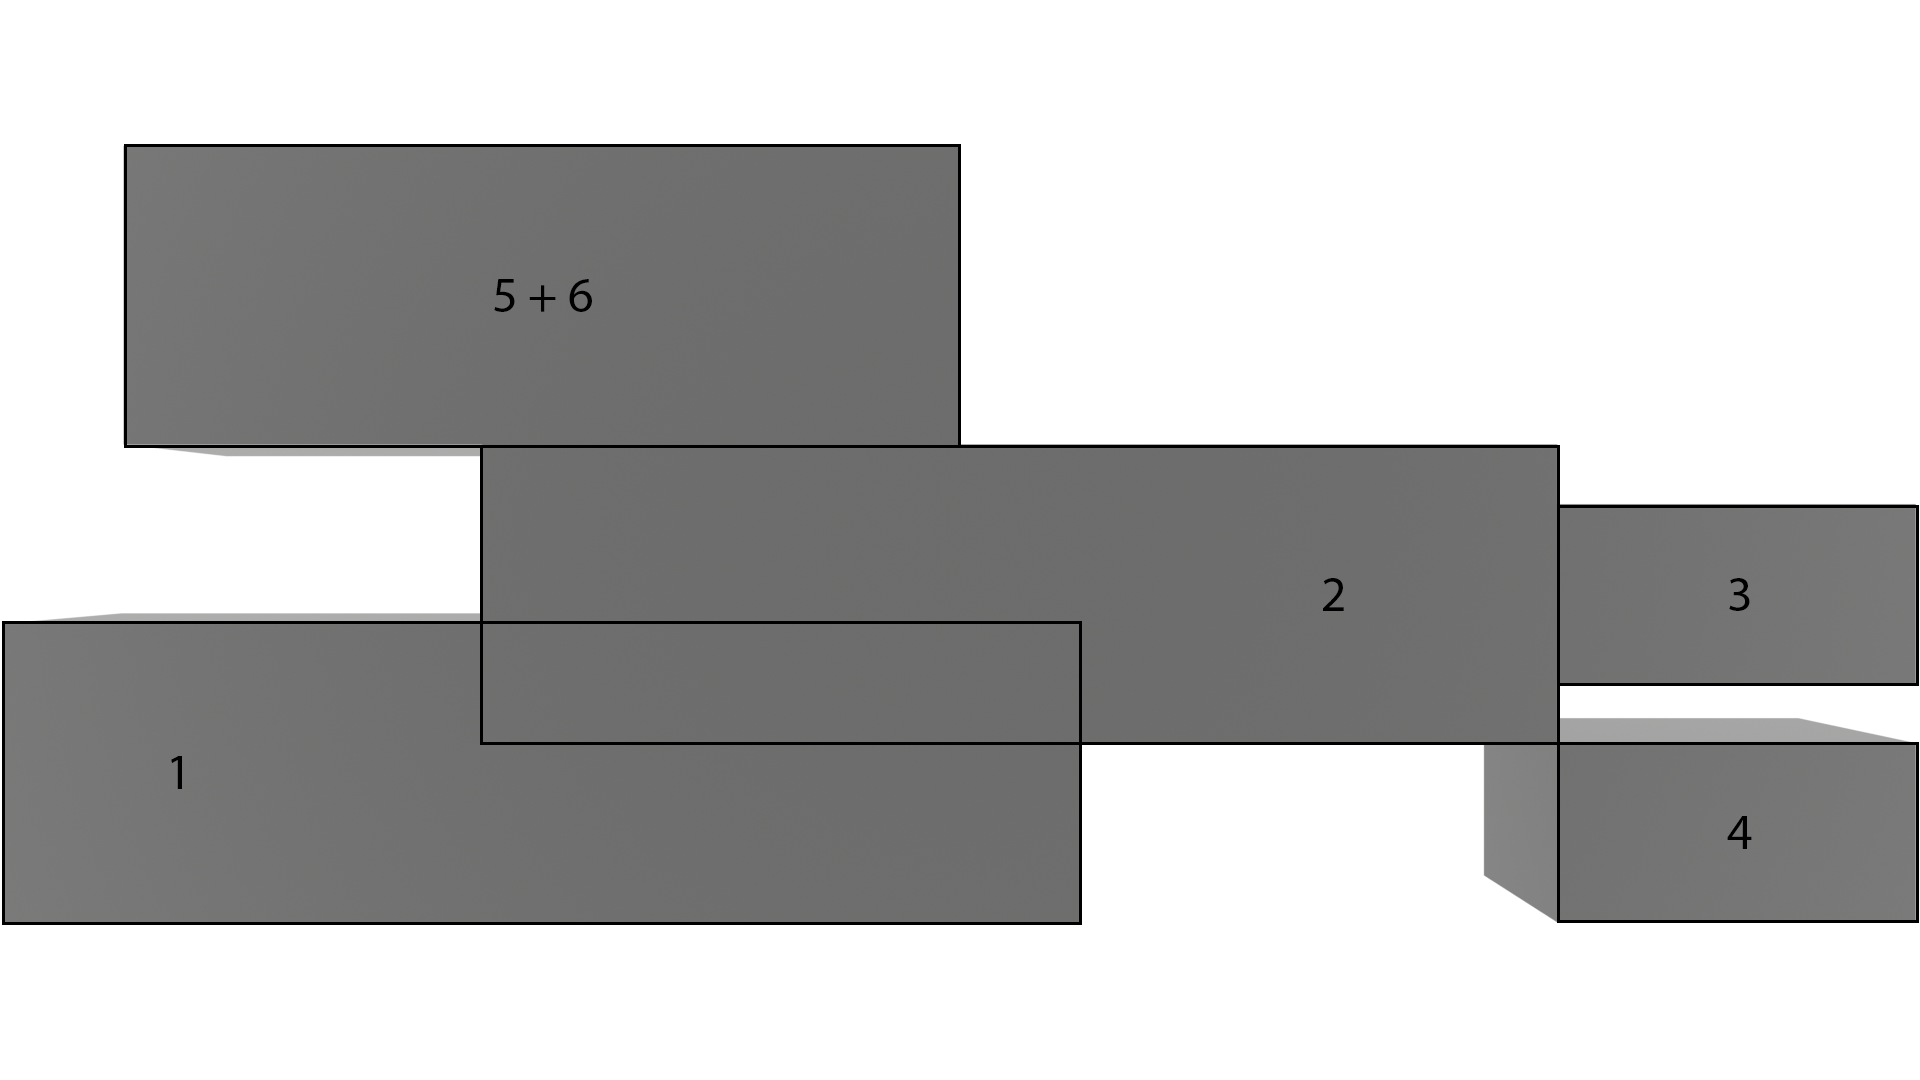
\includegraphics[width=0.8\columnwidth]{fig/Real_Combination_Base_labeled.png}
    \caption{Modell einer Wand, die durch 7 einzelne Wandstücke des selben Typs gebildet wird, deren Mittelpunkte alle auf einer Ebene liegen.}
    \label{fig:concept:combination_example_base}
\end{figure}

\paragraph*{Brigitten}\label{concept:combination_properties} sind alle Wandstücke,  die zwar in dem Modellierungsprozess des Gebäudes durch mehrere einzelne Wandstücke realisiert wurden, eigentlich aber eine Einheit darstellen. 
Es ist notwendig alle Wandstücke zu identifizieren, die einen zusammenhängenden Wandbereich bilden, um den gewählten Mauerwerksverband korrekt über alle Wandstücke hinweg anzuwenden.
Andernfalls würde jedes Wandstück den Mauerwerksverband unabhängig seiner Nachbarn neu beginnen und ihn dadurch zwischen Wandstückübergängen häufig fälschlicherweise unterbrechen.
Ein umfangreiches Beispiel ist in Abbildung~\ref*{fig:concept:combination_example_base} dargestellt.
Um zu überprüfen, ob zwei Wandstücke eine Einheit bilden, kann das Paar auf folgende Eigenschaften getestet werden:

\begin{enumerate}
    \item Beide Wandstücke verwenden das selbe Modul und sind während der Modellierung mit den gleichen Wandtyp annotiert worden. 
    Dies verhindert vor allem das Kombinieren unterschiedlich dicker Wände.
    \item\label{real:z_parallel} Die lokalen Z-Achsen beider Wandstücke sind parallel. 
    Dies verhindert das Kombinieren unpassend rotierter Wandstücke.
    Die Überprüfung der Parallelität der Z-Achsen beider Wandstücke wird wie folgt durchgeführt:

    Sei \(\vec{v}_z = {[0, 0, 1]}^T\)
    die Z-Achse und \(v_z = (v_w, v_x, v_y, v_z) = (0, 0, 0, 1)\) das dazugehörige Quaternion. 
    Außerdem seien \(q_1\) und \(q_2\) die beiden Rotationen der Wandstücke. Dann stellen 
    \(v_{z^1} = q_1 * v_z * q_1^{-1}\) und 
    \(v_{z^2} = q_2 * v_z * q_2^{-1}\) die jeweiligen \glqq{}Z-Anteile\grqq{} dieser Rotationen dar.
    Daraus ergeben sich die \glqq{}Z-Vektoren\grqq{} wie folgt: 
    \(\vec{v}_{z^1} = {[v_{z^1_x}, v_{z^1_y}, v_{z^1_z}]}^T\) und
    \(\vec{v}_{z^2} = {[v_{z^2_x}, v_{z^2_y}, v_{z^2_z}]}^T\).
    Ist nun \(|\vec{v}_{z^1} \cdot \vec{v}_{z^2}| = 1\) gegeben, so sind die lokalen Z-Achsen der Wandstücke gleich oder um exakt 180\degree{} verdreht und damit Parallelität erfüllt.
    \item Die lokalen X-Achsen beider Wandstücke sind ebenfalls parallel. Das Vorgehen zur Überprüfung entspricht dem von Punkt~\ref{real:z_parallel}, nur dass \(v_z\) durch \(v_x = (0, 1, 0, 0)\), also der X-Achse, ersetzt werden muss.
    \item Sie stehen auf der selben Höhe oder versetzt um ein Vielfaches der gemeinsamen Modulhöhe.
    \item\label{concept:schichten} Es liegt eine Berührung oder gar eine Überlappung vor.
\end{enumerate}

Insgesamt bilden in dem Beispiel in Abbildung~\ref{fig:concept:combination_example_base} demnach alle Wandstücke mit Ausnahme von Wandstück Nummer 4 eine Einheit, die alle obigen Eigenschaften erfüllt.
Dies sind in der Tat all die Wandstücke, die den Start des gewählten Mauerwerksverbands ihren Nachbarn anpassen müssen, sodass sich der Verband gleichmäßig über alle Wandstücke erstreckt.


\paragraph*{Ecken}
Der Grund dafür ist die Komplexität in diesen Bereichnen die vorgeschriebenen Normen (wie etwa dem in Abschnitt~\ref{basics:Mauerwerksverband} genannten Überbindemaß) einzuhalten.
Deswegen existieren für jeden Mauerwerksverband eigene spezielle Eck- und Kreuzungslegepläne, die an diesen Stellen eingefügt werden müssen.
Es werden wie oben nur diejenigen Wandstücke miteinander verglichen, die mit dem selben Wandtyp annotiert wurden und das gleiche Modul verwenden.
Da die drei Beziehungen sich stark ähneln, besitzen sie einige geteilte Eigenschaften:
\begin{enumerate}
    \item Die lokalen Z-Achsen beider Wandstücke sind parallel. Das Vorgehen zur Überprüfung ist dasselbe wie in Abschnitt~\ref{real:combination}.
    \item Sie stehen auf der selben Höhe oder versetzt um ein Vielfaches der gemeinsamen Modulhöhe.
    \item Mindestens eines der beiden Wandstücke endet auf einem anderen, sodass mindestens eine Schicht das andere Wandstück direkt berührt.
\end{enumerate}
Sind diese Eigenschaften erfüllt, werden für jede durch die einzelnen Schichten der Wandstücke vorgegebene Höhe Schnittpunkte zwischen den beiden Wandstücken errechnet.
Im Falle einer einfachen Ecke oder einer T-Kreuzung, existiert nur ein einzelnes Paar an Wandstücken, deren Schichten sich in jedem Höhenschritt des Moduls im Mittelpunkt der Ecke schneiden.
Der Unterschied ist lediglich die Stelle des Schnittpunkts relativ zu den beiden Wandstücken.
Liegt der errechnete Schnittpunkt bei beiden Wandstücken näher als Wandbreite/2 an einer der beiden Außenkanten handelt es sich um eine Ecke.
Falls der Schnittpunkt bei einem der beiden Wandstücke allerdings mindestens Wandbreite/2 innerhalb des Wandstücks liegt, so handelt es sich um eine T-Kreuzung.
Werden für zwei unterschiedliche Paare die selben Schnittpunkte errechnet, so kann es sich entweder um eine mit drei Wandstücken modellierte T-Kreuzung oder X-Kreuzung handeln.
Teilen sich zwei T-Kreuzungen die selben Schnittpunkte, so sind alle Vorraussetzungen für eine eine X-Kreuzung gegeben.
Liegt der Schnittpunkt des Wandstück-Paares mindesten Wandbreite/2 innerhalb beider Wandstücke, so handelt es sich um eine X-Kreuzung - modelliert aus zwei sich schneidenden Wandstücken. 
TODO Bilder

\paragraph*{T-Kreuzungen} 

\paragraph*{X-Kreuzungen}

\subsection*{Öffnungen}
Öffnungen ansprechen (vlt mit kleinem Diagramm?)


TODO Konzept hinter MaskedTransform und so erklkären
\section{Wall Detailing}
\label{concept:wall_detailing}
Als \glqq{}Wall Detailing\grqq{} (sprich das \glqq{}Detailieren von Wänden\grqq{}) wird in dieser Arbeit der Vorgang ein als geometrischer Körper definiertes Wandstück in ein konkretes Mauerwerk zu überführen, bezeichnet.


\section{Regelbasierte Bauplangenerierung}
blabla
